\documentclass[aps,prd,reprint,superscriptaddress,nofootinbib,longbibliography,floatfix]{revtex4-2}

\usepackage{amsmath,amssymb,mathtools}
\usepackage{bm}
\usepackage{booktabs}
\usepackage{array}
\usepackage{microtype}
\usepackage{graphicx}
\usepackage{tikz}
\usepackage{xcolor}
\usepackage{hyperref}
\usepackage{enumitem}
\usepackage{url}

% Slightly more open than the default REVTeX leading, while retaining
% the visual identity of the preceding TEF papers.
\linespread{1.06}\selectfont
\setlength{\parskip}{0.16em}
\setlist[itemize]{leftmargin=*,topsep=0.35em,itemsep=0.15em,parsep=0em}
\setlist[enumerate]{leftmargin=*,topsep=0.35em,itemsep=0.15em,parsep=0em}
\setlength{\emergencystretch}{2em}

\hypersetup{
  colorlinks=true,
  linkcolor=black,
  citecolor=black,
  urlcolor=blue,
  pdftitle={Closed Matter and Open Space: A Relative-Framing Ansatz for Incomplete Quark Sectors and the Matter-Space Interface},
  pdfauthor={Xiaodan Wu},
  pdfsubject={Version 4.6; DOI: 10.5281/zenodo.22256714}
}

\newcommand{\TEF}{\textsc{TEF}}
\newcommand{\ee}{\mathrm{e}}
\newcommand{\ii}{\mathrm{i}}
\newcommand{\Z}{\mathbb{Z}}
\newcommand{\Ustate}{\mathsf{U}}
\newcommand{\Dstate}{\mathsf{D}}
\newcommand{\Qem}{Q_{\mathrm{em}}}
\newcommand{\Cclosed}{\mathcal{C}_{\mathrm{closed}}}
\newcommand{\Sopen}{\mathcal{S}_{\mathrm{open}}}
\newcommand{\nufr}{\nu_{\mathrm{fr}}}

\begin{document}

\title{Closed Matter and Open Space:\\
A Relative-Framing Ansatz for Incomplete Quark Sectors\\
and the Matter--Space Interface}

\author{Xiaodan Wu}
\email{xiaodan@theemergentframe.org}
\affiliation{Independent Researcher}
\homepage{https://theemergentframe.org}
\thanks{ORCID: \href{https://orcid.org/0009-0005-5892-0293}{0009-0005-5892-0293}; DOI: \href{https://doi.org/10.5281/zenodo.22256714}{10.5281/zenodo.22256714}.}

\date{September 2, 2026 --- Version 4.6}

\begin{abstract}
The first three Emergent Frame (\TEF{}) preprints primarily explored the geometry of an open spatial sector through a gravity-calibrated circular-helix ansatz and conditional cross-sector correspondences. Paper IV addresses a different question. It adopts the working distinction that spatial properties may be governed primarily by geometry, whereas persistent matter may be governed primarily by closure and topology, and asks whether a mathematically explicit boundary language for a future interface between these descriptions can be formulated. Quark-like sectors are treated as locally persistent but globally incomplete sub-sectors of a closed matter configuration. For a fixed embedded open arc with a chosen normal-plane trivialization, a framing path $f:[0,1]\to S^1$ with fixed endpoint phase $\zeta$ has endpoint-fixed homotopy classes forming a torsor for $\pi_1(S^1)\cong\mathbb Z$. Thus relative class differences such as $\Delta w$ are well defined even though an absolute integer coordinate requires a reference choice. A separate threefold boundary postulate imposes $\zeta^3=1$ with $\zeta\neq1$; after an orientation choice, a selected adjacent pair can be designated $D/U$ with $\Delta w_{UD}=1$. Identifying the corresponding normalized framing lift with electric charge reproduces the familiar $-1/3$ and $+2/3$ classes, but that electromagnetic identification remains a physical postulate. The broader TEF conjecture is structural rather than helical: boundary-exposed matter sub-sectors may close into self-sustaining composites, while exposed or transferred boundary data may couple to an open-space sector. This provides a possible research bridge toward future closure energetics in the strong sector and, separately, relative-class-changing weak processes. Neither mechanism is derived here. Full $SU(3)_c$, a gauge-invariant charge construction, dynamics, Lorentz covariance, and fermionic quantization remain open. The result is therefore a pre-dynamical relative-framing ansatz for incomplete matter sectors and a proposed matter--space interface.
\end{abstract}

\maketitle

\section{Introduction}

The Standard Model classifies matter with extraordinary precision, but its characteristic discrete structures---fractional quark charge, color representations, chiral weak multiplets, and fermionic spinorial behavior---enter through representation data rather than a known microscopic topology \cite{PDG2026}. These facts do not require a deeper structural description; they provide constraints that any such description must survive.

The Emergent Frame (\TEF{}) program began from a spatial hypothesis: what is ordinarily treated as spacetime may itself be generated or organized by matter, and one candidate local geometry for the open spatial sector is a right-handed circular helix. Papers I--III explored that geometric branch and tested conditional correspondences with electroweak mixing, the fine-structure constant, and neutrino oscillation observables \cite{WuI,WuII,WuIII}. The present paper deliberately changes domain. It does not assume that every TEF question must be derived from the helix. Instead it develops a complementary working distinction that has emerged from the program: \emph{space may be characterized primarily by open geometry, whereas matter may be characterized primarily by closed or self-sustaining topology}. This is a research heuristic, not an established physical principle.

The motivation is the matter--space interface. A quark is never observed as an isolated asymptotic color state, while hadrons occur as color-singlet composites. In the present ansatz this motivates, but does not prove, the idea that a quark-like object is a locally persistent yet globally incomplete matter sub-sector. If such sub-sectors can close only as parts of larger composites, then the strong-interaction problem may be approached as an \emph{energetics of maintaining closure}: separating incomplete sectors would require an increasingly extended or reconfigured interface with the open spatial sector. Conversely, a weak transition that changes one local matter class may require the closed composite to exchange structural data with open modes. The paper is worth pursuing only if these ideas can be made more precise than analogy.

The strict mathematical step developed below is modest but concrete. A boundary-exposed framed matter sub-sector with fixed endpoint data has relative classes forming a $\mathbb Z$-torsor. This supplies a rigorous meaning to the statement that two local states can differ by one full relative-framing class without being treated as unrelated local structures. A threefold endpoint condition and the identification with quark charge remain additional postulates. The resulting construction is therefore neither a derivation of QCD nor a weak-interaction model; it is a first mathematical skeleton for the broader closed-matter/open-space hypothesis.

Topological particle models provide important precedents, especially twisted-ribbon and braid constructions \cite{BilsonThompson2005,BilsonThompson2007,Chester2025}. Triality also appears in modern algebraic organizations of Standard-Model representations \cite{FureyHughes2025}. The present work therefore makes no priority claim for topological charge encoding, three-strand structures, or triality. Its narrower purpose is to combine a rigorously defined relative-framing subsystem with the TEF hypothesis of globally incomplete quark sectors and to state how such sectors might interface with closed matter and open space.
\section{Logical status and scope}
\label{sec:ledger}

\begin{itemize}
\item \textbf{Established input.} Standard-Model quark charges, color triality, chiral weak currents, the absence of isolated color states from the asymptotic spectrum, and the possible global quotients of $SU(3)_c\times SU(2)_L\times U(1)_Y$.
\item \textbf{Mathematical result.} For a fixed open centerline with fixed endpoint framing data, $\pi_0(\mathcal P_\zeta)$ is a $\mathbb Z$-torsor; relative class differences such as $\Delta w$ are invariant under a common reference change.
\item \textbf{TEF matter-topology postulates.} A quark is a globally incomplete local sub-sector; a nontrivial threefold endpoint phase is imposed; one adjacent pair is designated $D/U$; and the normalized framing lift is identified with electric charge.
\item \textbf{TEF interface conjecture.} Closed matter and open space are structurally distinct sectors whose boundary data may be coupled. Strong-interaction research may test the energetics of maintaining closure, while the weak-sector conjecture concerns changes of local matter class that may be accompanied by exchange with open modes.
\item \textbf{Not derived.} Full $SU(3)_c$, confinement, a gauge-invariant electric-charge operator, an energy functional, Lorentz-covariant dynamics, anomaly consistency, weak transition amplitudes, and Finkelstein--Rubinstein fermionic quantization.
\end{itemize}

The construction should be revised or abandoned if no full three-dimensional configuration can embed the relative-framing subsystem while satisfying these physical constraints.
\section{From spatial geometry to matter topology}
\label{sec:continuity}

Papers I--III and the present paper belong to the same TEF program but address different structural layers. The earlier papers used a specific circular-helix geometry to probe the open spatial sector and froze its dimensionless shape parameter before carrying it across several conditional correspondence tests \cite{WuI,WuII,WuIII}. Paper IV does not reuse that parameter to determine quark charge, color, or weak quantum numbers, and the relative-framing theorem below does not require the centerline to be helical.

This independence is intentional rather than a defect. The current working picture is that geometry may be the natural language for the open spatial sector, while topology and closure may be the natural language for persistent matter. The two descriptions need not be identical. Their eventual unification, if any, should occur through a matter--space interface: boundary data of incomplete matter sectors, the way those sectors close into composites, and the way structural information can be exchanged with open spatial degrees of freedom.

Accordingly, Paper IV should not be read as a fourth attempt to extract a particle property from the frozen helix. It initiates a matter-topology and interface branch of the TEF program. Whether the specific helical geometry of Papers I--III eventually constrains a preferred framing, an energy functional, or an interface law remains an open coupling problem rather than a premise of the present construction.
\section{Standard-Model anchors}
\label{sec:anchors}

\subsection{First-generation quark charge and color triality}

For the first generation,
\begin{equation}
\Qem(u)=+\frac23e,
\qquad
\Qem(d)=-\frac13e,
\label{eq:udcharges}
\end{equation}
and both fields transform in the fundamental color representation \cite{PDG2026}. Their electric charges differ by one unit,
\begin{equation}
\Qem(u)-\Qem(d)=e.
\label{eq:chargedifference}
\end{equation}
It is useful to define a purely algebraic charge-class map
\begin{equation}
\chi(Q)\equiv\exp\!\left(2\pi\ii\frac{Q}{e}\right).
\label{eq:chargemap}
\end{equation}
This is not asserted to be an electromagnetic gauge holonomy; it only records electric charge modulo one unit. Equation~\eqref{eq:udcharges} then gives
\begin{equation}
\chi(Q_u)=\ee^{4\pi\ii/3}
=\ee^{-2\pi\ii/3}
=\chi(Q_d).
\label{eq:sameclass}
\end{equation}
Thus $u$ and $d$ occupy the same fractional electric-charge class while differing by one integer unit.

The center of $SU(3)$ is $\mathbb Z_3$. Let $N=N_q-N_{\bar q}$ denote the additive net number of fundamental quark sectors in a bookkeeping configuration, and define the corresponding center-triality class
\begin{equation}
\tau\equiv N\pmod3,
\qquad \tau\in\mathbb Z_3.
\label{eq:taudef}
\end{equation}
For a single quark, $N=1$ and $\tau=1$; for an antiquark, $N=-1$ and $\tau=-1\pmod3$. A color singlet is necessarily center-neutral, $\tau=0$, but the converse is false. For example, $3\otimes3\otimes3$ and $3\otimes\bar3$ both contain center-neutral nonsinglet representations in addition to singlets. The triality condition is therefore retained only as a coarse representation-level constraint, not as a color-singlet projector or a confinement mechanism \cite{PDG2026,Ghanbarpour2022}.

\subsection{Relation to the global form of the Standard Model gauge group}
\label{sec:globalSM}

The correlation between color-center data and Abelian charge assignments is not peculiar to TEF. The local Standard-Model gauge algebra admits several possible global forms,
\begin{equation}
G_{\rm SM,\Gamma}=
\frac{SU(3)_c\times SU(2)_L\times U(1)_Y}{\Gamma},
\qquad
\Gamma\subseteq\mathbb Z_6,
\label{eq:gsmglobal}
\end{equation}
with $\Gamma=1,\mathbb Z_2,\mathbb Z_3$, or $\mathbb Z_6$ compatible with the observed spectrum \cite{Tong2017,HsinGomis2024}. For the maximal $\mathbb Z_6$ quotient, a diagonal combination of the centers of $SU(3)$ and $SU(2)$ together with a hypercharge phase acts trivially on all Standard-Model multiplets. Consequently, the allowed non-Abelian center classes and $U(1)$ quantum numbers obey congruence conditions.

This mainstream group-theoretic background sharply limits the novelty claim of the present paper. The congruence
\begin{equation}
\boxed{\frac{\Qem}{e}\equiv-\frac{\tau}{3}\pmod1}
\label{eq:chargecongruence}
\end{equation}
for the restricted quark sector should be regarded first as a representation-level bookkeeping relation consistent with the known charge classes, not as a helical derivation of electric charge. The TEF-specific question is instead whether a concrete three-dimensional framed configuration can realize an analogous quotient or descent condition as an actual property of its configuration space and boundary data.

\subsection{Parallel weak doublets}

The first-generation left-handed fields form
\begin{equation}
Q_L=\begin{pmatrix}u_L\\ d_L\end{pmatrix},
\qquad
L_L=\begin{pmatrix}\nu_{eL}\\ e_L\end{pmatrix},
\label{eq:doublets}
\end{equation}
with $T_3=+1/2$ for the upper component and $T_3=-1/2$ for the lower component. Using the convention
\begin{equation}
\frac{\Qem}{e}=T_3+\frac{Y}{2},
\label{eq:smcharge}
\end{equation}
the left-handed quark doublet has $Y=1/3$ and the lepton doublet has $Y=-1$ \cite{PDG2026}. Define
\begin{equation}
b\equiv T_3+\frac12\in\{0,1\}.
\label{eq:bindex}
\end{equation}
Then
\begin{align}
\frac{\Qem}{e}&=b-\frac13,
&&Q_L,\label{eq:qbinary}\\
\frac{\Qem}{e}&=b-1,
&&L_L.\label{eq:lbinary}
\end{align}
These equations contain no new Standard-Model physics. They expose only a two-state ordering in the left-handed weak sector. The right-handed quarks $u_R$ and $d_R$ are $SU(2)_L$ singlets with $T_3=0$; therefore any later identification of the intrinsic $U/D$ label with $b$ must be restricted to the left-handed doublet and cannot serve as a universal definition of quark type.

\section{A restricted relative-framing ansatz}
\label{sec:ansatz}

We now separate the speculative TEF assumptions from the established anchors above.

\subsection{Postulate A: quarks are globally incomplete matter sectors}

A quark is not modeled as an independently closed microscopic object. It is instead a locally persistent sector of a larger matter configuration. The additive bookkeeping variable is
\begin{equation}
N\equiv N_q-N_{\bar q}\in\mathbb Z,
\label{eq:Ndef}
\end{equation}
while only
\begin{equation}
\tau=N\bmod3
\label{eq:taumod}
\end{equation}
represents the $\mathbb Z_3$ color-center class. This separation removes the ambiguity that would arise if an arbitrary integer lift of triality were itself treated as physical. Center neutrality, $\tau=0$, remains only a necessary representation-level condition for a physical color singlet.

\subsection{Boundary-exposed framed matter sub-sector and a general endpoint phase}

To convert the phase-lift label into a precise relative-homotopy problem, let $\gamma:[0,1]\to\mathbb R^3$ be any fixed embedded arc and let $\mathbf n(s)$ be a continuous unit vector in its normal plane. The torsor result below does not require $\gamma$ to be helical. In the present paper this is deliberate: the framed arc is a candidate boundary-exposed matter sub-sector, not a geometric model of the open spatial carrier itself. Choosing a smooth reference trivialization $(\mathbf e_1(s),\mathbf e_2(s))$ of the normal bundle along the arc, the framing can be written as
\begin{equation}
\mathbf n(s)=\cos\theta(s)\,\mathbf e_1(s)+\sin\theta(s)\,\mathbf e_2(s),
\label{eq:framingvector}
\end{equation}
or equivalently by the $S^1$-valued phase
\begin{equation}
f(s)=e^{i\theta(s)}\in S^1.
\label{eq:framingphase}
\end{equation}
No ribbon width or additional length scale is required; the ribbon picture is only a visualization of the framing direction.

We first keep the endpoint phase general. Write
\begin{equation}
f(0)=1,
\qquad
f(1)=\zeta=e^{2\pi i a},
\qquad a\in\mathbb R/\mathbb Z,
\label{eq:generalzeta}
\end{equation}
and define the endpoint-fixed path space
\begin{equation}
\mathcal P_{\zeta}
\equiv
\left\{
 f:[0,1]\to S^1\,\middle|\,f(0)=1,\ f(1)=\zeta
\right\}.
\label{eq:Pzeta}
\end{equation}
Two paths are equivalent when they are homotopic through paths that keep both endpoints fixed.

\subsection{Standard proposition: relative-framing classes form a $\mathbb Z$-torsor}

The set $\pi_0(\mathcal P_\zeta)$ of endpoint-fixed homotopy classes is a torsor for
\begin{equation}
\pi_1(S^1,1)\cong\mathbb Z.
\label{eq:pi1S1}
\end{equation}
This is a standard consequence of covering-space and fundamental-groupoid theory, applied here to the chosen relative-framing subsystem \cite{Brown2006,KoSmolinsky1992}.

To exhibit the action explicitly, let
\begin{equation}
\ell_k(s)=e^{2\pi i k s},
\qquad k\in\mathbb Z,
\label{eq:loopk}
\end{equation}
be a loop based at $1$. Because $S^1$ is a group, pointwise multiplication defines
\begin{equation}
(k\cdot f)(s)\equiv \ell_k(s)f(s),
\qquad
k\cdot[f]\equiv[k\cdot f].
\label{eq:torsoraction}
\end{equation}
Since $\ell_k(0)=\ell_k(1)=1$, the endpoint conditions are preserved. The action is free and transitive: for any two endpoint-fixed classes there is a unique $k\in\mathbb Z$ carrying one to the other.

\emph{Proof.} Let $p:\mathbb R\to S^1$, $p(\vartheta)=e^{i\vartheta}$, be the universal covering map. Choose a real representative $a$ of the endpoint phase in Eq.~\eqref{eq:generalzeta}. Every $f\in\mathcal P_\zeta$ has a unique lift $\widetilde\theta:[0,1]\to\mathbb R$ with $\widetilde\theta(0)=0$, and its endpoint must satisfy
\begin{equation}
\widetilde\theta(1)=2\pi(a+w),
\qquad w\in\mathbb Z.
\label{eq:liftendpointgeneral}
\end{equation}
Endpoint-fixed homotopy preserves the lifted endpoint. Conversely, if two lifts $\widetilde\theta_0$ and $\widetilde\theta_1$ have the same endpoints, the linear homotopy
\begin{equation}
H(s,t)=(1-t)\widetilde\theta_0(s)+t\widetilde\theta_1(s)
\label{eq:lifthomotopy}
\end{equation}
keeps both endpoints fixed, and $p\circ H$ gives an endpoint-fixed homotopy of the original paths. Pointwise multiplication by $\ell_k$ shifts the lifted endpoint by $2\pi k$, so Eq.~\eqref{eq:torsoraction} is free and transitive. Hence $\pi_0(\mathcal P_\zeta)$ is an affine copy, or torsor, of $\mathbb Z$. \hfill$\square$

The proposition supplies the mathematical step missing in Version 3, but its scope is deliberately narrow. It applies to a fixed centerline with fixed endpoint framing data inside the explicitly stipulated subsystem $\mathcal P_\zeta$. It does not classify the full configuration space of a deformable three-dimensional field, and homotopy disconnection does not by itself imply a dynamical energy barrier, stability, conservation law, or transition amplitude.

\subsection{Dependence on trivialization and reference framing}
\label{sec:trivialization}

The path coordinate $f=e^{i\theta}$ is defined only after choosing a normal-plane trivialization. If the reference frame is changed by a rotation $\alpha(s)$,
\begin{equation}
(\mathbf e'_1,\mathbf e'_2)=R_{\alpha(s)}(\mathbf e_1,\mathbf e_2),
\label{eq:framechange}
\end{equation}
then the same physical framing vector has coordinate
\begin{equation}
\theta'(s)=\theta(s)-\alpha(s),
\qquad
f'(s)=e^{-i\alpha(s)}f(s).
\label{eq:phasetransform}
\end{equation}
After re-normalizing the initial phase to unity, the endpoint mismatch is measured as
\begin{equation}
\zeta'
=e^{-i[\alpha(1)-\alpha(0)]}\zeta.
\label{eq:zetatransform}
\end{equation}
Thus $\zeta$ is not an intrinsic comparison of two different normal-plane fibers until a trivialization, connection, parallel-transport rule, or physically defined endpoint identification has been specified.

A particularly instructive case occurs when the primed and unprimed frames agree as rotations at both endpoints but the lifted reference frame itself winds $k$ times along the interval, so that
\begin{equation}
\alpha(1)-\alpha(0)=2\pi k.
\label{eq:alphawinding}
\end{equation}
The endpoint phase on $S^1$ is unchanged, while the lifted integer coordinate shifts as
\begin{equation}
w\longmapsto w-k.
\label{eq:wshift}
\end{equation}
Accordingly, the torsor structure and differences such as $\Delta w$ are independent of a common change of reference, whereas an absolute assignment such as $w=0$ requires a chosen torsor origin. A future physical model must supply a preferred frame, connection, or gauge-invariant equivalent. No preferred framing is derived here from the spatial geometry used in Papers I--III.

\subsection{Postulate B: a nontrivial threefold endpoint mismatch}

We now add a TEF-specific boundary condition to the general construction. The endpoint phase is required to obey
\begin{equation}
\zeta^3=1,
\qquad
\zeta\neq1.
\label{eq:zetaBC}
\end{equation}
Choosing one orientation convention gives
\begin{equation}
\zeta=e^{-2\pi i/3},
\qquad
a=-\frac13\pmod1.
\label{eq:zetachoice}
\end{equation}
The conjugate primitive root $\zeta^{-1}=e^{+2\pi i/3}$ reverses this boundary phase. The physical motivation is that one sector is globally incomplete while three identical sector endpoint phases multiply to the identity. This is a TEF matter-boundary postulate, not a consequence of the torsor theorem and not a derivation of the three colors of QCD.

Combining Eq.~\eqref{eq:liftendpointgeneral} with Eq.~\eqref{eq:zetachoice} gives, in the chosen orientation, trivialization, and torsor-origin convention,
\begin{equation}
\widetilde\theta(1)
=-\frac{2\pi}{3}+2\pi w,
\qquad w\in\mathbb Z.
\label{eq:liftendpoint}
\end{equation}
Topology supplies the integer-spaced torsor; the fractional offset is supplied by the imposed threefold endpoint phase.

\begin{figure}[!ht]
\centering
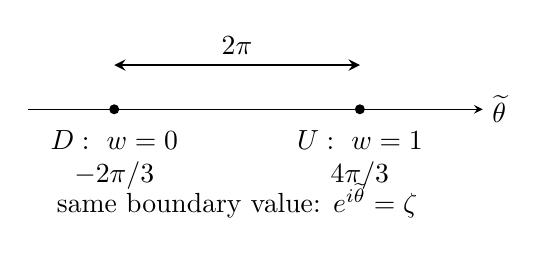
\begin{tikzpicture}[x=0.78cm,y=0.78cm,>=stealth]
  \draw[->] (-0.3,0) -- (7.1,0) node[right] {$\widetilde\theta$};
  \fill (1.1,0) circle (1.8pt);
  \fill (5.1,0) circle (1.8pt);
  \node[below=4pt,align=center] at (1.1,0) {$D:\ w=0$\\$-2\pi/3$};
  \node[below=4pt,align=center] at (5.1,0) {$U:\ w=1$\\$4\pi/3$};
  \draw[<->,thick] (1.1,0.72) -- node[above] {$2\pi$} (5.1,0.72);
  \node[below] at (3.1,-1.05) {same boundary value: $e^{i\widetilde\theta}=\zeta$};
\end{tikzpicture}
\caption{Universal-cover view after choosing the threefold endpoint phase and a torsor origin. The selected adjacent classes designated $D$ and $U$ have lifted endpoint angles differing by $2\pi$ but project to the same endpoint-framing phase $\zeta$ on $S^1$. The labels $w=0,1$ are coordinate choices on the torsor; the invariant statement is $\Delta w_{UD}=1$.}
\label{fig:relativeframing}
\end{figure}

\subsection{Postulate C: $D$ and $U$ are a chosen adjacent pair}

After choosing a torsor origin, we designate one adjacent pair of relative-framing classes as the first-generation quark types,
\begin{equation}
\Dstate:\quad w=0,
\qquad
\Ustate:\quad w=1,
\qquad
\Delta w_{UD}=1.
\label{eq:UDclasses}
\end{equation}
There is no mathematically lowest class in the torsor. The reason that the physical low-energy spectrum would select this pair rather than additional classes $w=-1,2,\ldots$ is an unresolved dynamical question for a future energy functional.

Their lifted endpoint angles are
\begin{align}
\widetilde\theta_D(1)&=-\frac{2\pi}{3},
\label{eq:Dangle}\\
\widetilde\theta_U(1)&=-\frac{2\pi}{3}+2\pi
=\frac{4\pi}{3},
\label{eq:Uangle}
\end{align}
while their endpoint-framing phases agree,
\begin{equation}
e^{i\widetilde\theta_D(1)}
=e^{i\widetilde\theta_U(1)}
=\zeta.
\label{eq:sameendpointphase}
\end{equation}
Thus the selected $D$ and $U$ classes have the same boundary value $\zeta$ but differ by one full relative-framing turn. That distinction is invariant under the stipulated endpoint-fixed homotopies in the fixed-centerline subsystem; no dynamical stability is inferred from this fact alone.

\subsection{Postulate D: framing-lift coordinate and electric charge}

Define, within the chosen convention, the dimensionless normalized framing-lift coordinate
\begin{equation}
\nufr
\equiv
\frac{\widetilde\theta(1)}{2\pi}
=w-\frac13.
\label{eq:nufr}
\end{equation}
Equation~\eqref{eq:nufr} follows \emph{conditionally} from the imposed threefold endpoint phase, the orientation choice, the chosen normal-plane trivialization, and the chosen torsor origin. Under a common reference-frame winding its absolute integer part shifts as in Eq.~\eqref{eq:wshift}, whereas differences between classes do not. This symbol is unrelated to the frozen helix shape parameter $q=a/R$ used in Papers I--III.

To connect the construction to particle physics we introduce the separate physical identification
\begin{equation}
\boxed{\frac{Q_{\rm em}}{e}=\nufr.}
\label{eq:chargeidentification}
\end{equation}
Then, in the selected convention,
\begin{align}
\Dstate:&\quad Q_{\rm em}/e=-\frac13,
\label{eq:Dcharge}\\
\Ustate:&\quad Q_{\rm em}/e=+\frac23.
\label{eq:Ucharge}
\end{align}
The distinction in logical status is essential: topology supplies the relative integer spacing; Postulate B supplies the fractional offset; Eq.~\eqref{eq:chargeidentification} supplies the electromagnetic interpretation. Electromagnetic $U(1)$, its connection, coupling, Gauss law, and charge quantization have not been derived. A complete theory must also make the absolute charge assignment independent of arbitrary reference-framing choices.

\subsection{Conjugation and composite boundary multiplication}

The $S^1$ framing admits a natural phase-conjugation map
\begin{equation}
C(f)(s)=\overline{f(s)}=f(s)^{-1},
\label{eq:conjugation}
\end{equation}
which sends
\begin{equation}
C:\mathcal P_\zeta\longrightarrow\mathcal P_{\zeta^{-1}}.
\label{eq:Cmap}
\end{equation}
If a quark lift has endpoint $2\pi(a+w)$, the conjugate path has endpoint $2\pi(-a-w)$. With compatible torsor-origin conventions this implements
\begin{equation}
a\mapsto-a,
\qquad
w\mapsto-w,
\qquad
\nufr\mapsto-\nufr.
\label{eq:conjugatelift}
\end{equation}
For the chosen threefold phase, this reproduces the opposite fractional phase classes. It is only an Abelian framing-phase conjugation; it does not construct the full $3\to\bar3$ color representation, quantum-field charge conjugation, chirality transformation, or CPT.

For several sectors whose phases are expressed in a common $U(1)$ framing fiber with compatible parameterization and trivialization, define pointwise group multiplication
\begin{equation}
F(s)=
\prod_{i=1}^{N_q} f_i(s)
\prod_{j=1}^{N_{\bar q}} g_j(s),
\qquad g_j\in\mathcal P_{\zeta^{-1}}.
\label{eq:compositeF}
\end{equation}
Equivalently, taking each antiquark endpoint phase to be $\zeta^{-1}$, the composite boundary value is
\begin{equation}
F(1)=\zeta^{N_q-N_{\bar q}}=\zeta^N,
\qquad
N=N_q-N_{\bar q}.
\label{eq:compositeendpoint}
\end{equation}
Thus $N=0\pmod3$ gives a trivial Abelian boundary phase for the imposed cubic root. This multiplication is the coarse boundary bookkeeping used below; it is not path concatenation and it does not establish a full $SU(3)_c$ singlet, Gauss-law constraint, or confinement mechanism. Additive lift coordinates such as $W=\sum_i w_i$ are meaningful only after compatible reference choices have been made across sectors.

\section{Threefold phase structure: triality clue, not color closure}
\label{sec:closure}

The construction imposes
\begin{equation}
\zeta^3=1,
\qquad
\zeta=e^{-2\pi i/3},
\label{eq:zetaclosure}
\end{equation}
so three identical sector endpoint phases multiply to the identity. The familiar roots-of-unity relation $1+\omega+\omega^2=0$ is only a secondary geometric picture; it is not a color model. All three QCD basis colors belong to the same fundamental $SU(3)_c$ representation, and the $\mathbb Z_3$ center acts with the same center phase on the entire triplet. A genuine microscopic theory must therefore embed any threefold boundary structure into continuous $SU(3)_c$ rather than replace color by three fixed phases.

This novelty boundary is important because twisted-ribbon models already encode fractional charge and color-related data topologically, and recent algebraic work organizes Standard-Model representations using triality \cite{BilsonThompson2005,Chester2025,FureyHughes2025}. The present claim is narrower: the imposed threefold endpoint phase is combined with a relative-framing torsor so that a selected $D/U$ pair differs by one integer class. The threefold phase itself is not claimed as a new discovery.

\section{Composite-sector bookkeeping}
\label{sec:composites}

For three quark sub-sectors, $N=3$ and $\tau=0$. With compatible torsor origins and trivializations, the charge identification gives the sanity check
\begin{equation}
\frac{Q_B}{e}=W-1=N_U-1,
\qquad W=\sum_{i=1}^{3}w_i,
\label{eq:baryoncharge}
\end{equation}
so the selected $DDD,UDD,UUD,UUU$ assignments reproduce the familiar charges $-1,0,+1,+2$ by construction. This is not a prediction. Likewise a quark--antiquark pair has $N=0$ and a trivial Abelian boundary phase. Neither condition is sufficient for a physical color singlet, since
\begin{equation}
3\otimes\bar3=1\oplus8,
\qquad
3\otimes3\otimes3=1\oplus8\oplus8\oplus10.
\label{eq:colorproducts}
\end{equation}
The construction therefore supplies only triality-level boundary bookkeeping, not a singlet projector, Gauss law, or confinement mechanism.

\section{Matter closure and the open-space interface}
\label{sec:interface}

The original motivation for Paper IV is broader than the $D/U$ framing pair. It is the possibility that persistent matter and open space correspond to different structural regimes of the same underlying physics: matter is self-sustaining only when its local boundary data close consistently, whereas open spatial degrees of freedom need not form such closed configurations. The present paper does not define an ontological substrate common to both. It only asks whether a useful boundary language can connect them.

Three distinct objects must therefore be kept separate. First, $\mathcal Q[D]$ or $\mathcal Q[U]$ denotes a \emph{boundary-exposed framed matter sub-sector} carrying the relative class discussed above. Second, $\Cclosed[\cdots]$ denotes a \emph{closed composite matter configuration} in which the exposed data of its constituent sub-sectors are internally matched. Third, $\Sopen[\cdots]$ denotes a conjectural \emph{open-space/propagating mode sector}. The boundary-exposed matter sub-sector and the open-space/propagating mode sector are not asserted to be the same object; this distinction is retained explicitly throughout.

At the coarse $U(1)$ boundary level already defined in Sec.~\ref{sec:ansatz}, a collection of sub-sectors with boundary phases $\zeta_i$ has the product
\begin{equation}
B_{\rm tot}=\prod_i\zeta_i.
\label{eq:boundaryproduct}
\end{equation}
The condition $B_{\rm tot}=1$ is only Abelian boundary closure/triality bookkeeping. It is not a substitute for a color-singlet projector, but it gives a concrete prototype of what ``closure'' means in the restricted construction: individually nontrivial boundary data can cancel or match in the composite.

\subsection{Strong-sector research direction: energetics of closure}

The absence of isolated color states and the approximately linear growth of the static heavy-quark potential over the confining regime provide an established QCD benchmark \cite{PDG2026}. In full QCD with dynamical quarks, string breaking limits the literal extension of that potential, so no simple classical-string identification is assumed here. The TEF conjecture is instead structural: if a quark-like sub-sector is globally incomplete, separating such sectors while preserving a closed composite may require an increasingly extended or reconfigured interface with open spatial degrees of freedom. A future energy functional could then ask whether the cost of maintaining closure reproduces any aspect of confining dynamics.

The appropriate future question is therefore energetic rather than merely topological: given an admissible closed composite configuration, how does the minimum energy compatible with its closure boundary conditions change under separation or deformation of its incomplete sub-sectors? No energy functional, string tension, running coupling, flux tube, or strong-coupling constant is calculated in the present paper. The point is only to identify a concrete pressure test for a later strong-interaction model.

\subsection{Weak-sector conjecture: relative-class-changing exchange}

For the left-handed quark doublet only, the Standard-Model binary index $b=T_3+1/2$ has the same ordering as the selected relative-framing pair,
\begin{equation}
w=b=T_3+\frac12,
\qquad (Q_L\ \text{only}),
\label{eq:wisb}
\end{equation}
so $d_L$ corresponds to the designated class $w=0$ and $u_L$ to $w=1$. This is only a left-handed algebraic correspondence; $u_R$ and $d_R$ are weak singlets. The full charged current contains CKM and PMNS mixing,
\begin{equation}
J_+^\mu=
\bar u_{Li}\gamma^\mu V_{ij}d_{Lj}
+\bar\nu_{Lk}U^*_{\alpha k}\gamma^\mu e_{L\alpha},
\label{eq:chargedcurrent}
\end{equation}
so first-generation notation is a simplifying limit \cite{PDG2026}.

At energies well below $m_W$, beta decay contains the effective structure
\begin{equation}
\mathcal L_{\rm eff}^{(\beta)}\propto
V_{ud}(\bar u_L\gamma^\mu d_L)
(\bar e_L\gamma_\mu\nu_{eL})+\mathrm{h.c.}
\label{eq:betaeff}
\end{equation}
The TEF conjecture is that a change of local matter class may be accompanied by exchange with open-space modes. With $X$ denoting unchanged spectator sub-sectors, this is represented only schematically as
\begin{equation}
\Cclosed[\Dstate;X]
\longrightarrow
\Cclosed[\Ustate;X]
+\Sopen[e^-,\bar\nu_e].
\label{eq:closedopen}
\end{equation}
This is not a transition operator or QFT vertex. It indicates the type of matter--space interface that a future microscopic theory would need to define. Electron and neutrino remain distinct asymptotic states; the weaker conjecture is that they may be described as distinct modes within the conjectural open-space/propagating sector rather than each being modeled as an independently closed matter topology. Purely leptonic decay, neutral-current neutrino scattering, chirality, flavor mixing, and the full $W$-mediated structure remain pressure tests.

Taken together, the strong and weak directions suggest a possible division of labor rather than a claimed unification: strong dynamics may test how closure is maintained and energetically stressed, while weak dynamics may test how a closed configuration changes class and exchanges structure with open-space modes. Whether either interpretation survives a full field theory is an open question.
\section{Relation to earlier topological and gauge-structure work}
\label{sec:literature}

The closest topological precedent is the Helon/braided-ribbon program, in which ribbon twists encode electric-charge data and braids encode additional particle structure \cite{BilsonThompson2005,BilsonThompson2007,Chester2025}. The present relative-framing construction is therefore not a claim that twist-based charge encoding is new. Its distinctive element is the conditional combination of a boundary-exposed matter sub-sector, an imposed threefold endpoint phase, an adjacent-class torsor structure, and the proposal that closure data are the point of contact with an open spatial sector.

The charge--triality congruence also has a mainstream group-theoretic background. The Standard Model admits global gauge groups
\begin{equation}
G=\frac{SU(3)_c\times SU(2)_L\times U(1)_Y}{\Gamma},
\qquad
\Gamma=1,\mathbb Z_2,\mathbb Z_3,\mathbb Z_6,
\end{equation}
and the choice of quotient correlates non-Abelian center data with Abelian quantum numbers \cite{Tong2017,HsinGomis2024}. The present construction is therefore only \emph{compatible with} such discrete structure; it does not derive the Standard-Model global form.

Finally, Finkelstein--Rubinstein-type quantization of soliton configuration spaces shows how nontrivial loops can generate fermionic signs \cite{KruschSpeight2006}. This remains a future criterion here: the $\mathbb Z$ torsor of an open framing path has not been identified with the loop produced by a physical $2\pi$ spatial rotation.

\section{Embedding problem beyond the restricted subsystem}
\label{sec:framed}

The proven torsor statement concerns only a fixed open strand with fixed endpoint framing data. Framed braid theory similarly records integer strand framings, but a physical matter model would require a much larger configuration space in which local sub-sectors deform, join into closed composites, couple to open spatial degrees of freedom, and gauge-equivalent descriptions are identified \cite{KoSmolinsky1992}. For closed framed ribbons, a useful precedent is
\begin{equation}
Lk=Tw+Wr,
\label{eq:CWF}
\end{equation}
the C\u{a}lug\u{a}reanu--White--Fuller relation, which shows how local twist and global writhe can combine into a topological invariant \cite{White1969,Fuller1971}. Whether the present open-sector class difference embeds into an analogous invariant of a closed composite is unknown.

If $D$ and $U$ are represented by adjacent classes, a change $\Delta w=\pm1$ cannot occur through an endpoint-fixed homotopy of $\mathcal P_\zeta$. It must leave that restricted path space by changing boundary data, reconnecting, passing through a singular configuration, or exchanging data with another sector. This is a statement about the stipulated subsystem, not evidence for a weak-interaction mechanism.

No mass parameter is used to label the classes. A future local action would have to determine the energies of its finite-energy configurations and explain why only the observed adjacent pair is relevant at low energy; $E_{\rm rest}=mc^2$ is merely the standard conversion from rest energy to observed mass. Such a theory must also address Derrick-type stability, Lorentz covariance, continuous $SU(3)_c$, electromagnetic gauge structure, chiral weak couplings, anomaly cancellation, and fermionic quantization \cite{Derrick1964}.

The imposed $2\pi/3$ endpoint mismatch and the $2\pi$ torsor generator now inhabit the same $S^1$ framing space. The familiar $4\pi$ fermionic behavior remains separate: the parity map $w\mapsto w\bmod2$ is not a derivation of spin-$1/2$. A full configuration space would have to identify the physical rotation and exchange loops and implement the appropriate Finkelstein--Rubinstein sign character.

\section{Discussion and conclusion}

Paper IV marks a change of structural question within the TEF program. Papers I--III primarily explored a candidate geometry of the open spatial sector. The present work asks instead whether persistent matter can be organized by topology and closure, and whether the boundary between incomplete matter sectors and open spatial degrees of freedom can provide a common language for later interaction models. The paper therefore does not require its strict mathematical result to depend on the circular helix used previously.

The concrete construction is intentionally limited. For a fixed boundary-exposed framed matter sub-sector with fixed endpoint data, the path components of $\mathcal P_\zeta$ form a $\mathbb Z$-torsor. A selected $D/U$ pair can therefore differ intrinsically by one relative class, $\Delta w_{UD}=1$, even though the absolute labels $w=0,1$ require a reference framing and torsor origin. The fractional offset $\zeta=e^{-2\pi i/3}$ is a separate threefold matter-boundary postulate, and the identification $Q_{\rm em}/e=\nufr$ is a further physical postulate. The construction therefore organizes known quark-charge classes; it does not derive electric charge or $SU(3)_c$.

The broader reason for retaining this ansatz is the closed-matter/open-space interface. In the restricted boundary bookkeeping, individually incomplete sub-sectors can combine so that their exposed phase data close. This suggests two distinct future tests. In the strong sector, one may ask whether an energy functional for maintaining such closure under separation or deformation can reproduce any aspect of confinement or the observed scale dependence of strong interactions. In the weak sector, one may ask whether a change between adjacent local matter classes can be represented as a relative-class-changing process that exchanges structural data with open-space modes. Neither mechanism is established here, but both arise from the same structural question: what distinguishes a self-sustaining closed matter configuration from an open spatial excitation, and how can one be transformed into the other?

This framing also clarifies the relation to the earlier helical work. The helix remains one candidate geometry for the open spatial sector, but no direct derivation of the matter-boundary phase from helical transport is assumed or required in this paper. Such a derivation would constitute a future result of an independently motivated matter--space coupling law, rather than a premise of the present construction. Any future relation between the two branches must therefore come from such a coupling law, not from forcing matter topology to inherit every feature of the spatial geometry.

The next substantive step is therefore an embedding problem. A full theory must provide a three-dimensional configuration space containing the relative-framing subsystem, a physically meaningful closure operation, an energy functional, gauge and Lorentz structure, and a quantization rule. Only then can the proposed interface be tested against confinement, weak amplitudes, fermionic statistics, and particle spectra. Until that point, the present result is best read as a pre-dynamical matter-topology ansatz with an explicit relative-framing construction and a clearly stated bridge to the strong- and weak-interaction research programs.
\begin{acknowledgments}
The author thanks the researchers whose work on precision Standard Model phenomenology, QCD triality, topological particle models, soliton quantization, and emergent gauge structure provides the constraints against which this exploratory construction can be tested.
\end{acknowledgments}

\begin{thebibliography}{99}

\bibitem{WuI}
X.~Wu,
``A Helical Spacetime Ansatz Linking the Planck Scale and Electroweak Mixing,''
Version 5.1 (2026), Zenodo,
\href{https://doi.org/10.5281/zenodo.22101000}{doi:10.5281/zenodo.22101000}.

\bibitem{WuII}
X.~Wu,
``From a Gravity-Calibrated Helix to a Conditional Fine-Structure Correspondence,''
Version 4.7 (2026), Zenodo,
\href{https://doi.org/10.5281/zenodo.22117153}{doi:10.5281/zenodo.22117153}.

\bibitem{WuIII}
X.~Wu,
``From a Gravity-Calibrated Helix to Neutrino Oscillation Correspondences: A Third Cross-Sector Comparison of the Frozen TEF Shape Parameter,''
Version 4.2 (2026), Zenodo,
\href{https://doi.org/10.5281/zenodo.22150998}{doi:10.5281/zenodo.22150998}.

\bibitem{PDG2026}
F.~Takahashi \textit{et al.} (Particle Data Group),
``Review of Particle Physics,''
\textit{Int. J. Mod. Phys. A} \textbf{41}, 2630011 (2026),
\href{https://doi.org/10.1142/S0217751X26300115}{doi:10.1142/S0217751X26300115}.

\bibitem{BilsonThompson2005}
S.~O.~Bilson-Thompson,
``A Topological Model of Composite Preons,''
arXiv:hep-ph/0503213 (2005).

\bibitem{BilsonThompson2007}
S.~O.~Bilson-Thompson, F.~Markopoulou, and L.~Smolin,
``Quantum Gravity and the Standard Model,''
\textit{Class. Quantum Grav.} \textbf{24}, 3975--3993 (2007),
\href{https://doi.org/10.1088/0264-9381/24/16/002}{doi:10.1088/0264-9381/24/16/002}.

\bibitem{Chester2025}
D.~Chester, X.~D.~Arsiwalla, and L.~H.~Kauffman,
``Preons, Braid Topology, and Representations of Fundamental Particles,''
\textit{Int. J. Theor. Phys.} \textbf{64}, 221 (2025),
\href{https://doi.org/10.1007/s10773-025-06087-2}{doi:10.1007/s10773-025-06087-2};
arXiv:2501.03260.

\bibitem{Ghanbarpour2022}
M.~Ghanbarpour and L.~von Smekal,
``Quarks and Triality in a Finite Volume,''
\textit{Phys. Rev. D} \textbf{106}, 054513 (2022),
\href{https://doi.org/10.1103/PhysRevD.106.054513}{doi:10.1103/PhysRevD.106.054513};
arXiv:2206.11697.

\bibitem{FureyHughes2025}
N.~Furey and M.~J.~Hughes,
``Three Generations and a Trio of Trialities,''
\textit{Phys. Lett. B} \textbf{865}, 139473 (2025),
\href{https://doi.org/10.1016/j.physletb.2025.139473}{doi:10.1016/j.physletb.2025.139473};
arXiv:2409.17948.

\bibitem{KruschSpeight2006}
S.~Krusch and J.~M.~Speight,
``Fermionic Quantization of Hopf Solitons,''
\textit{Commun. Math. Phys.} \textbf{264}, 391--410 (2006),
\href{https://doi.org/10.1007/s00220-005-1469-4}{doi:10.1007/s00220-005-1469-4}.

\bibitem{Tong2017}
D.~Tong,
``Line Operators in the Standard Model,''
J. High Energy Phys. \textbf{07}, 104 (2017),
\href{https://doi.org/10.1007/JHEP07(2017)104}{doi:10.1007/JHEP07(2017)104};
arXiv:1705.01853.

\bibitem{HsinGomis2024}
P.-S.~Hsin and J.~Gomis,
``Detecting Standard Model Gauge Group from Generalized Fractional Quantum Hall Effect,''
arXiv:2411.18160 (2024).


\bibitem{KoSmolinsky1992}
K.~H.~Ko and L.~Smolinsky,
``The Framed Braid Group and 3-Manifolds,''
\textit{Proc. Am. Math. Soc.} \textbf{115}, 541--551 (1992),
\href{https://doi.org/10.1090/S0002-9939-1992-1126197-1}{doi:10.1090/S0002-9939-1992-1126197-1}.

\bibitem{Brown2006}
R.~Brown,
\textit{Topology and Groupoids}, 3rd ed. (BookSurge, 2006),
ISBN 1-4196-2722-8.

\bibitem{White1969}
J.~H.~White,
``Self-Linking and the Gauss Integral in Higher Dimensions,''
\textit{Am. J. Math.} \textbf{91}, 693--728 (1969),
\href{https://doi.org/10.2307/2373348}{doi:10.2307/2373348}.

\bibitem{Fuller1971}
F.~B.~Fuller,
``The Writhing Number of a Space Curve,''
\textit{Proc. Natl. Acad. Sci. USA} \textbf{68}, 815--819 (1971),
\href{https://doi.org/10.1073/pnas.68.4.815}{doi:10.1073/pnas.68.4.815}.

\bibitem{Derrick1964}
G.~H.~Derrick,
``Comments on Nonlinear Wave Equations as Models for Elementary Particles,''
\textit{J. Math. Phys.} \textbf{5}, 1252--1254 (1964),
\href{https://doi.org/10.1063/1.1704233}{doi:10.1063/1.1704233}.

\end{thebibliography}

\end{document}
